\documentclass[10pt]{scrartcl}

\usepackage[T1]{fontenc}
\usepackage{amssymb, amsmath, amsthm}
\usepackage{geometry, graphicx, enumitem, wrapfig, fancyhdr,cancel, physics}
\usepackage[english]{babel}
\usepackage{mlmodern}

% \usepackage{listings, xcolor}
% \definecolor{codegreen}{rgb}{0,0.6,0}
% \definecolor{codegray}{rgb}{0.5,0.5,0.5}
% \definecolor{codepurple}{rgb}{0.58,0,0.82}
% \definecolor{backcolour}{rgb}{0.95,0.95,0.92}

% \lstdefinestyle{mystyle}{
%     backgroundcolor=\color{backcolour},   
%     commentstyle=\color{codegreen},
%     keywordstyle=\color{magenta},
%     numberstyle=\tiny\color{codegray},
%     stringstyle=\color{codepurple},
%     basicstyle=\ttfamily\footnotesize,
%     breakatwhitespace=false,         
%     breaklines=true,                 
%     captionpos=b,                    
%     keepspaces=true,                 
%     numbers=left,                    
%     numbersep=5pt,                  
%     showspaces=false,                
%     showstringspaces=false,
%     showtabs=false,                  
%     tabsize=4
% }
% \lstset{style=mystyle}
\geometry{a4paper, margin=0.8in}
\pagestyle{fancy}
\lhead{PH3204 - Experiment 1}
\rhead{Debayan Sarkar \texttt{22MS002}}
\everymath{\displaystyle}
\theoremstyle{definition}
\newtheorem{exercise}{Question}
\newenvironment{solution} {\begin{proof}[\normalfont \textbf{Solution}]} {\end{proof}}

\renewcommand{\qedsymbol}{}
\newcommand{\nn}{\mathbb{N}}
\newcommand{\npixL}{\frac{n\pi x}{L}}
\newcommand{\rn}{\mathbb{R}}
\newcommand{\q}{\mathbb{Q}}
\newcommand{\p}{\mathcal{P}}
\newcommand{\z}{\mathbb{Z}}
\newcommand{\dx}{\mathrm{d}x}
\newcommand*{\OO}{\hat{O}}
\newcommand*{\Op}{\hat{p}}
\newcommand*{\Ox}{\hat{x}}
\newcommand*{\OH}{\hat{H}}
\newcommand*{\Oa}{\hat{a}}
\title{Study of the Zener diode as a voltage regulator and the use of IC 7805 as a voltage stabilizer}  
\subtitle{PH3204 - Electronics Laboratory}
\author{Debayan Sarkar \\ \texttt{22MS002}}
\date{\today}

\geometry{a4paper, margin=1in}
\setlength{\parindent}{0pt}
\begin{document}
\maketitle
\section{Introduction}
In this experiment we have studied the properties of a Zener Diode, under varying input and output signals.
Later, we also used the LM7805 IC to see the voltage stabilizer in action.
\subsection{Zener Diode}
A Zener Diode is a special type of Diode that is typically operated in Reverse Bias. It is designed
to allow current to flow "backwards" when a certain amount of reverse voltage is reached. Because of
this property, it can be used as a voltage regulator in circuits.

The Zener diode's operation depends on the heavy doping of its p–n junction. 
The depletion region formed in the diode is very thin and hence the electric field is 
very high even for a small reverse bias voltage, allowing electrons to 
tunnel from the valence band of the p-type material to the conduction band of the n-type 
material.
\subsection{LM7805 Regulator}
In the second part of the experiment, we replaced the Zener Diode with a dedicated Voltage Regulator
Integrated Circuit. We used the LM7805 Regulator, which is a member of the 78xx series of fixed
linear voltage regulators. Below you can see the 7805 Voltage Regulator Pin Diagram.

\begin{figure}[!h]
    \centering
    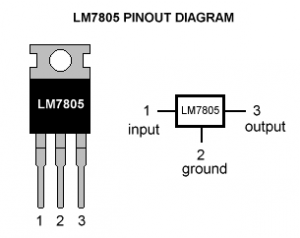
\includegraphics[width=0.3\linewidth]{IC.png}
    \caption{LM7805 Regulator Pinout (Souce: The Internet)}
\end{figure}

Here's a small description for each of the pins.
\begin{enumerate}
    \item \textbf{INPUT: }Input voltage (7V-35V)
    \item \textbf{GROUND: }Ground (0V)
    \item \textbf{OUTPUT: }Regulated output; 5V (4.8V-5.2V)
    
\end{enumerate}
\clearpage
\subsection{Experimental Setup}
The circuit for this experiment was prepared on a breadboard.
Below is the Circuit Diagram for the setup used in this experiment.

\begin{figure}[!h]
    \centering
    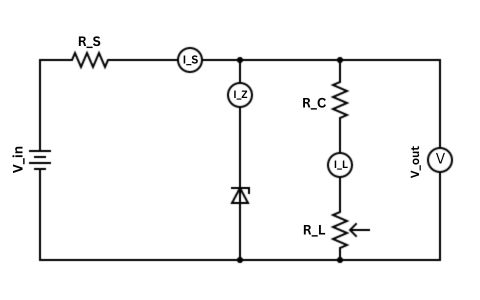
\includegraphics[width=0.6\linewidth]{circuit.png}
    \caption{Circtuit Diagram of the Setup}
\end{figure}
Where, 
\begin{itemize}
    \item $V_{in}$ is the input voltage (0 - 15 V) being produced using a DC Power Supply.
    \item $R_S = 2.2 k\Omega$
    \item $I_S$ is the total current flowing in the circuit being measured using a DT-830D multimeter.
    \item $I_Z$ is the total current flowing through the Zener Diode (or LM7805 IC) being measured using a DT-830D multimeter.
    \item $I_L$ is the load current, being measured using a DT-830D multimeter.
    \item $R_C = 2.2 \text{ (or $1$)} k\Omega$
    \item $R_L = 0 \text{ to } 1 k\Omega$ is a potentiometer.
    \item $V_{out}$ is the output voltage being measured using a 8007 multimeter. Note that this is also
        the voltage drop across the Diode.
\end{itemize}

\clearpage
\section{Studying a Zener Diode}
In this part of the experiment, we studied the properties of the given Zener Diode.
\subsection{Line Regulation}
In this part of the experiment, we varied the input voltage ($V_{in}$) from 0 to 15 Volts
with a constant load resistance of $R_c = 2.2 k\Omega$. 
\subsubsection{Data}
\begin{table}[!ht]
    \centering
    \caption{Line Regulation data for the Zener Diode}
    \begin{tabular}{|c|c|c|c|c|c|}
    \hline
        \textbf{$R_L$ ($k\Omega$)} & \textbf{$R_c$} & \textbf{$V_{in}$ (V)} & \textbf{$I_s$ (mA)} & \textbf{$I_z$ (mA)} & \textbf{$V_{out}$ (V)} \\ \hline
        0 & 2.2 & 0 & 0 & 0 & 0 \\ \hline
        0 & 2.2 & 0.5 & 0.094 & 0 & 0.298 \\ \hline
        0 & 2.2 & 1 & 0.187 & 0 & 0.592 \\ \hline
        0 & 2.2 & 1.49 & 0.279 & 0 & 0.88 \\ \hline
        0 & 2.2 & 1.99 & 0.373 & 0 & 1.177 \\ \hline
        0 & 2.2 & 2.5 & 0.469 & 0 & 1.473 \\ \hline
        0 & 2.2 & 2.99 & 0.559 & 0 & 1.76 \\ \hline
        0 & 2.2 & 3.5 & 0.653 & 0.001 & 2.06 \\ \hline
        0 & 2.2 & 3.9 & 0.749 & 0.003 & 2.35 \\ \hline
        0 & 2.2 & 4.51 & 0.848 & 0.007 & 2.65 \\ \hline
        0 & 2.2 & 5.04 & 0.953 & 0.021 & 2.93 \\ \hline
        0 & 2.2 & 5.52 & 1.058 & 0.048 & 3.18 \\ \hline
        0 & 2.2 & 5.99 & 1.174 & 0.095 & 3.39 \\ \hline
        0 & 2.2 & 6.48 & 1.307 & 0.164 & 3.58 \\ \hline
        0 & 2.2 & 7.01 & 1.464 & 0.263 & 3.75 \\ \hline
        0 & 2.2 & 7.5 & 1.622 & 0.375 & 3.88 \\ \hline
        0 & 2.2 & 7.99 & 1.79 & 0.501 & 3.98 \\ \hline
        0 & 2.2 & 8.48 & 1.966 & 0.643 & 4.07 \\ \hline
        0 & 2.2 & 8.99 & 2.21 & 0.868 & 4.18 \\ \hline
        0 & 2.2 & 9.49 & 2.4 & 1.038 & 4.24 \\ \hline
        0 & 2.2 & 10 & 2.61 & 1.218 & 4.29 \\ \hline
        0 & 2.2 & 10.51 & 2.81 & 1.403 & 4.34 \\ \hline
        0 & 2.2 & 11.02 & 3.02 & 1.595 & 4.39 \\ \hline
        0 & 2.2 & 11.51 & 3.22 & 1.784 & 4.42 \\ \hline
        0 & 2.2 & 12.01 & 3.43 & 1.972 & 4.45 \\ \hline
        0 & 2.2 & 12.5 & 3.63 & 2.39 & 4.48 \\ \hline
        0 & 2.2 & 12.98 & 3.93 & 2.59 & 4.53 \\ \hline
        0 & 2.2 & 13.52 & 4.17 & 2.82 & 4.55 \\ \hline
        0 & 2.2 & 14.02 & 4.39 & 3.05 & 4.58 \\ \hline
        0 & 2.2 & 14.51 & 4.6 & 3.27 & 4.6 \\ \hline
        0 & 2.2 & 15 & 4.84 & 3.5 & 4.61 \\ \hline
    \end{tabular}
\end{table}
\clearpage
\subsubsection{Analysis}
Below is are the plots generated from the above data.

\begin{figure}[h]
    \centering
    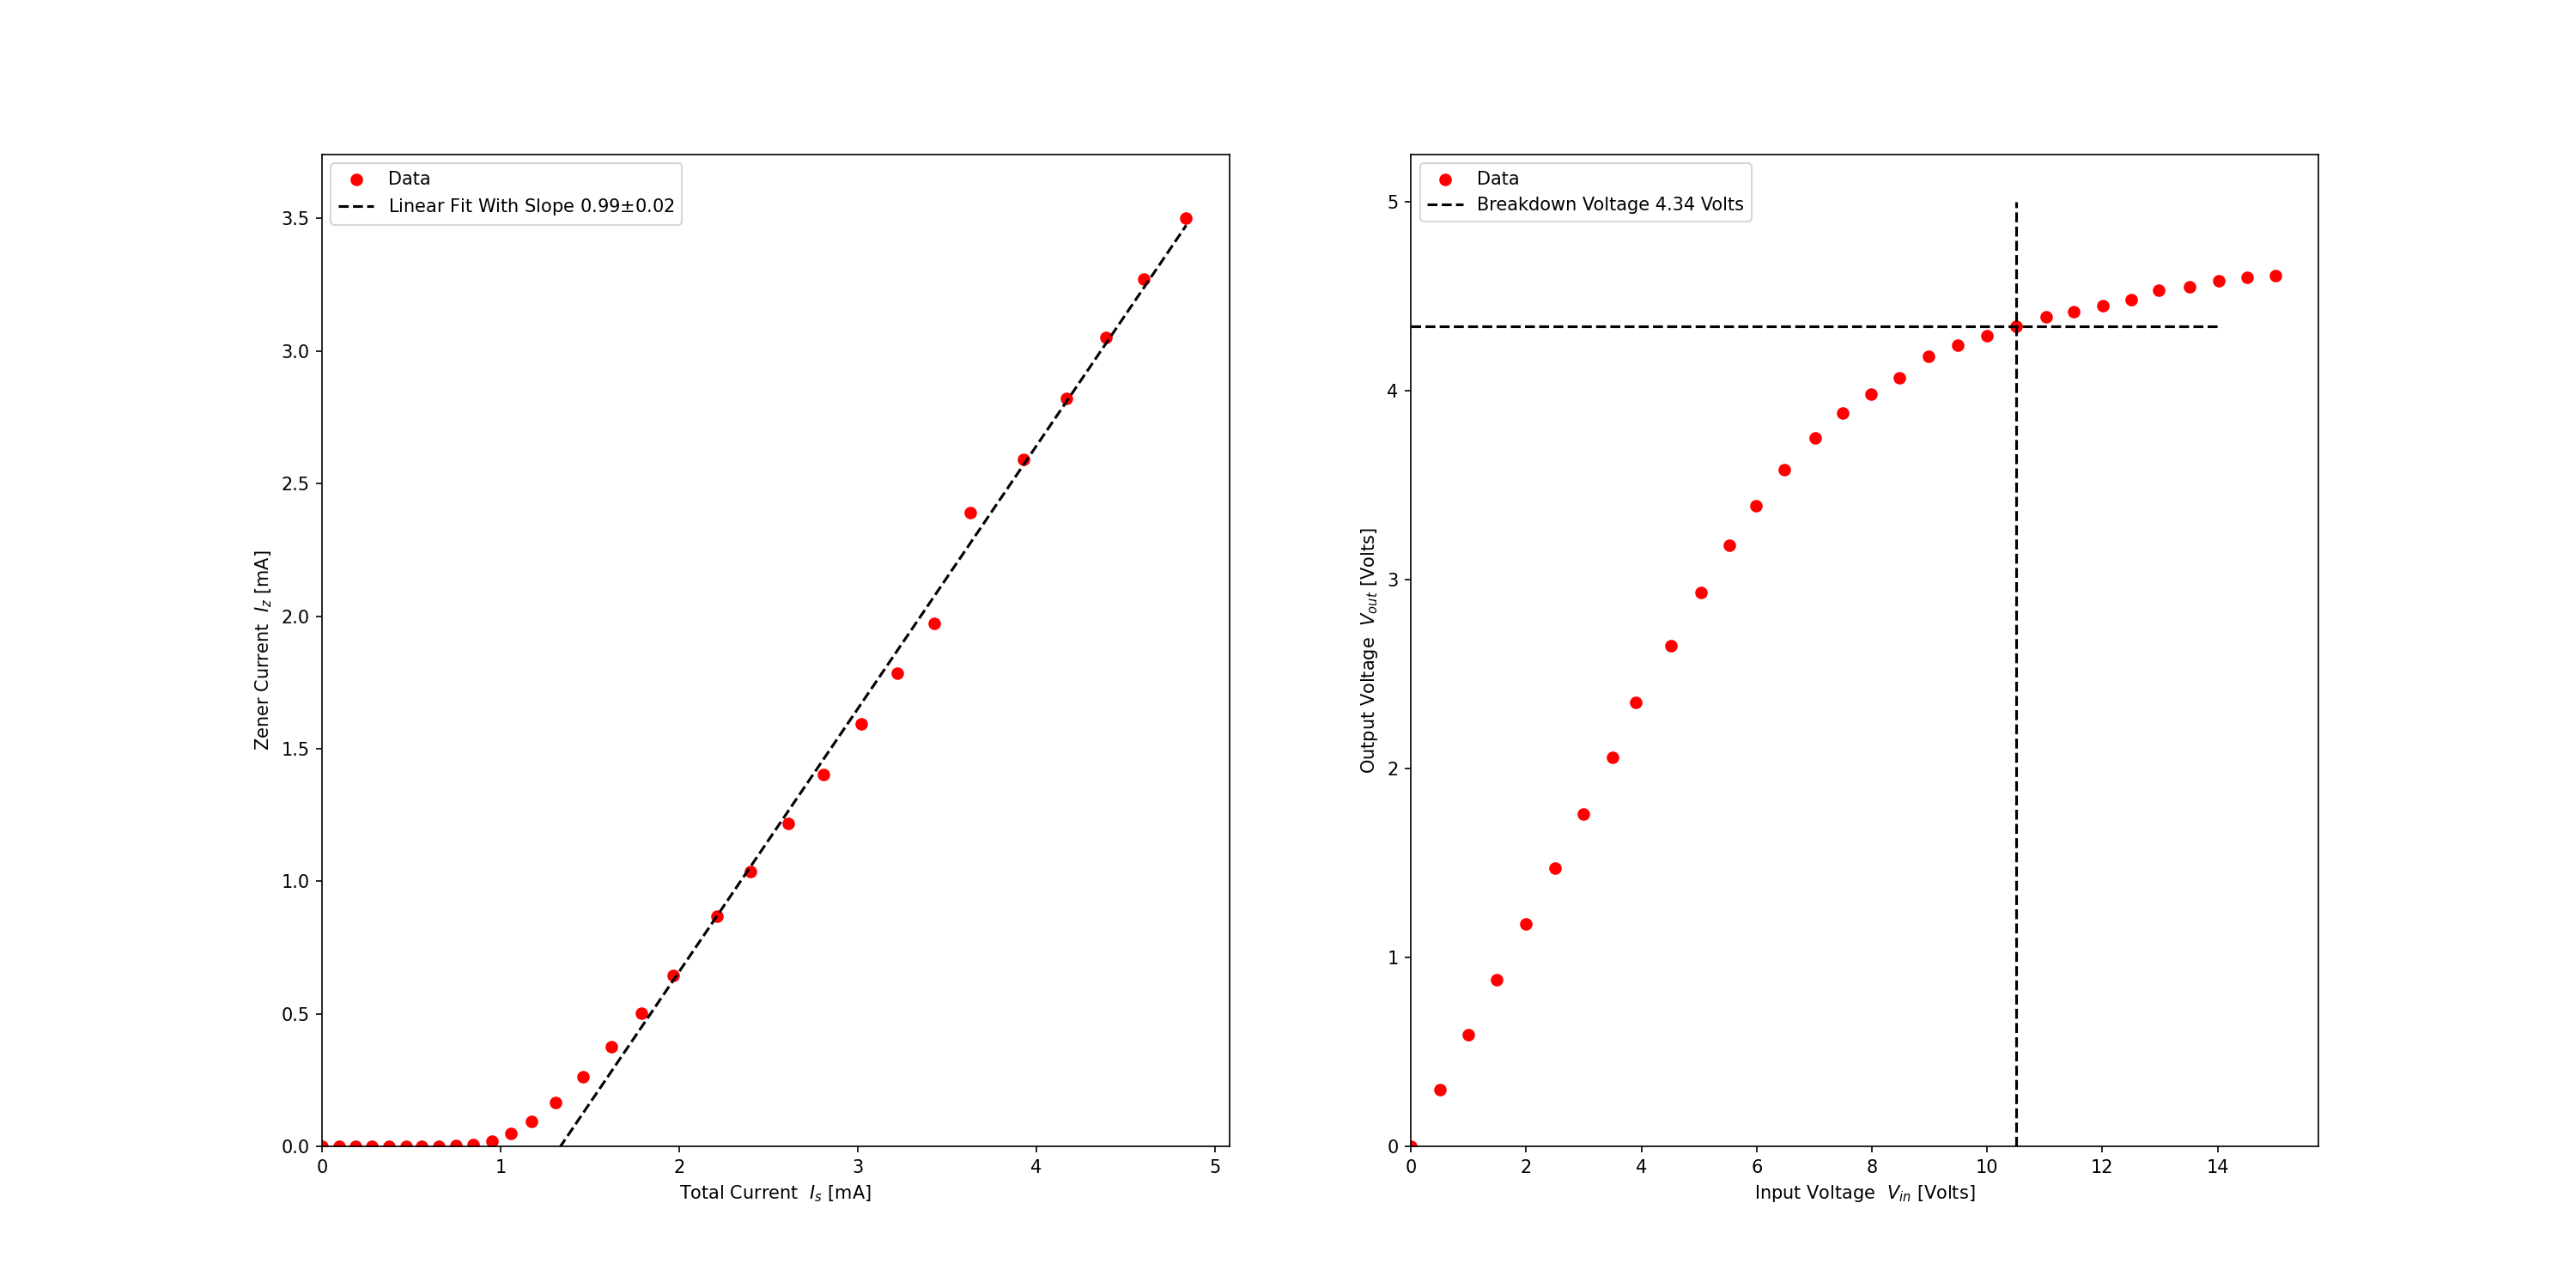
\includegraphics[width=\linewidth]{linereg.png}
    \caption{Plots of the Zener Diode data}
\end{figure}
From the plots, we can see that the graph between $I_z$ and $I_s$ is approximately a straight line
after reaching a threshold voltage. From the fit for the $I_z$ vs $I_s$ plot we can see that
\begin{align*}
    &\frac{\delta{I_z}}{\delta{I_s}} = 0.99 \pm 0.02 \\ 
    \Rightarrow &\boxed{\delta{I_z} = (0.99 \pm 0.02)\delta{I_s}}
\end{align*}
From the $V_{in}$ vs $V_{out}$ plot we can see that \textbf{Zener Breakdown} is occurring at $\boxed{V_{out} = 4.34 V}$
\subsection{Load Regulation}
In this part of the experiment, we kept the input voltage $V_{in}$ constant at 15 Volts, and changed the
Load Resistance, using a potentiometer.
\clearpage
\subsubsection*{$R_c = 1 k\Omega$}
\subsubsection{Data}
\begin{table}[!h]
    \centering
    \caption{Load Regulation data for the Zener Diode with $R_c = 1 k\Omega$}
    \begin{tabular}{|c|c|c|c|c|}
    \hline
        \textbf{$V_{in}$ (V)} & \textbf{ $R_L$ ($k\Omega$)} & \textbf{$I_L$ (mA)} & \textbf{$I_z$ (mA)} & \textbf{$V_{out}$(V)} \\ \hline
        15 & 1.45 & 4.15 & 0 & 6.03 \\ \hline
        15 & 1.473 & 4.13 & 0 & 6.07 \\ \hline
        15 & 1.486 & 4.12 & 0 & 6.1 \\ \hline
        15 & 1.492 & 4.11 & 0 & 6.12 \\ \hline
        15 & 1.497 & 4.1 & 0 & 6.14 \\ \hline
        15 & 1.521 & 4.09 & 0 & 6.16 \\ \hline
        15 & 1.528 & 4.07 & 0.01 & 6.18 \\ \hline
        15 & 1.584 & 4.06 & 0.02 & 6.22 \\ \hline
        15 & 1.563 & 4.03 & 0.02 & 6.26 \\ \hline
        15 & 1.583 & 3.98 & 0.04 & 6.34 \\ \hline
        15 & 1.626 & 3.96 & 0.05 & 6.35 \\ \hline
        15 & 1.616 & 3.95 & 0.06 & 6.36 \\ \hline
        15 & 1.661 & 3.88 & 0.1 & 6.41 \\ \hline
        15 & 1.967 & 3.29 & 0.67 & 6.44 \\ \hline
        15 & 2.04 & 3.16 & 0.8 & 6.46 \\ \hline
    \end{tabular}
\end{table}
\subsubsection{Analysis}
Below are the plots generated from the above data.

\begin{figure}[h]
    \centering
    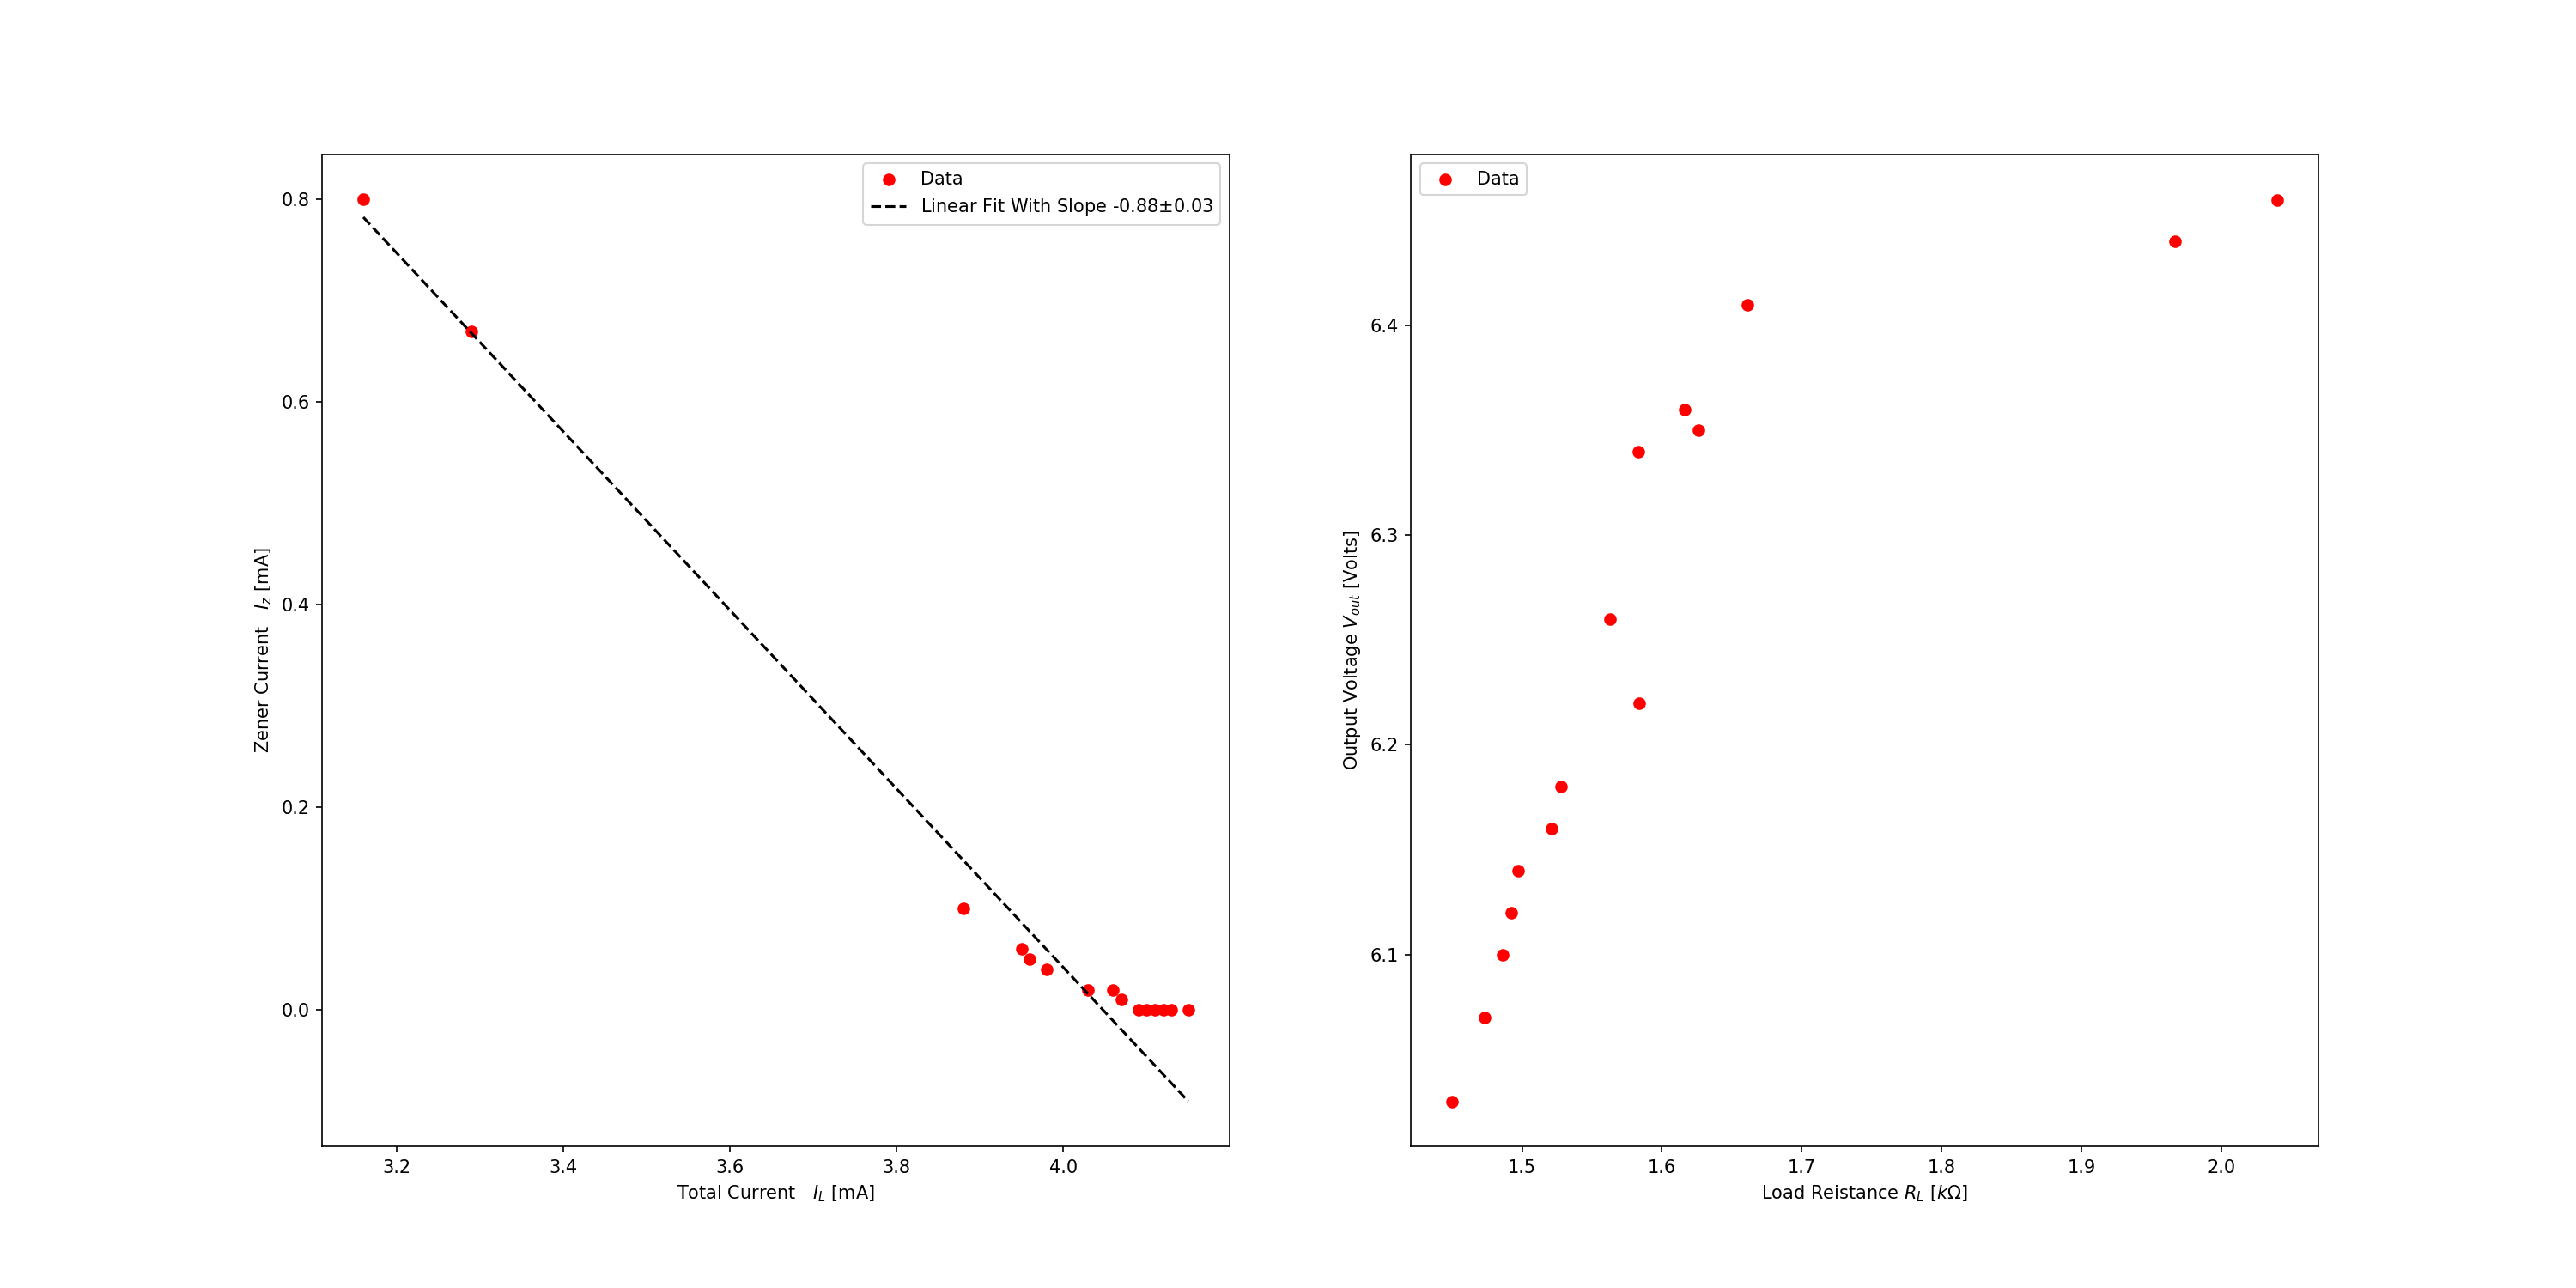
\includegraphics[width=\linewidth]{withoutrc.png}
    \caption{Plots of the Zener Diode load regulation data with $R_c = 1 k\Omega$}
\end{figure}
As we can see in the above plots, we havent reached the breakdown voltage yet, since the Load resistance
is too small. We can see however, just like in the previous section, 
\begin{align*}
    &\frac{\delta{I_z}}{\delta{I_s}} = -0.88 \pm 0.03 \\ 
    \Rightarrow &\boxed{\delta{I_z} = (-0.88 \pm 0.03)\delta{I_s}}
\end{align*}
\subsubsection*{$R_c = 2.2 k\Omega$}
\subsubsection{Data}
\begin{table}[!h]
    \centering
    \caption{Load Regulation data for the Zener Diode with $R_c = 2.2 k\Omega$}
    \begin{tabular}{|c|c|c|c|c|}
    \hline
        \textbf{$V_{in}$ (V)} & \textbf{ $R_L$ ($k\Omega$)} & \textbf{$I_L$ (mA)} & \textbf{$I_z$ (mA)} & \textbf{$V_{out}$(V)} \\ \hline
        15 & 0 & 2.1 & 2.89 & 4.56 \\ \hline
        15 & 0.034 & 2.08 & 2.93 & 4.56 \\ \hline
        15 & 0.071 & 2.05 & 2.95 & 4.57 \\ \hline
        15 & 0.106 & 2.02 & 3.01 & 4.57 \\ \hline
        15 & 0.126 & 2 & 3.02 & 4.58 \\ \hline
        15 & 0.17 & 1.96 & 3.06 & 4.58 \\ \hline
        15 & 0.195 & 1.94 & 3.08 & 4.58 \\ \hline
        15 & 0.232 & 1.91 & 3.11 & 4.58 \\ \hline
        15 & 0.274 & 1.88 & 3.13 & 4.59 \\ \hline
        15 & 0.305 & 1.86 & 3.15 & 4.59 \\ \hline
        15 & 0.323 & 1.84 & 3.17 & 4.59 \\ \hline
        15 & 0.359 & 1.82 & 3.19 & 4.59 \\ \hline
        15 & 0.387 & 1.8 & 3.22 & 4.59 \\ \hline
        15 & 0.435 & 1.77 & 3.24 & 4.59 \\ \hline
        15 & 0.473 & 1.72 & 3.33 & 4.6 \\ \hline
        15 & 0.561 & 1.69 & 3.3 & 4.6 \\ \hline
        15 & 0.633 & 1.65 & 3.34 & 4.6 \\ \hline
        15 & 0.721 & 1.6 & 3.37 & 4.6 \\ \hline
        15 & 0.826 & 1.55 & 3.44 & 4.61 \\ \hline
        15 & 0.919 & 1.48 & 3.53 & 4.62 \\ \hline
        15 & 1.025 & 1.45 & 3.53 & 4.62 \\ \hline
    \end{tabular}
\end{table}
\subsubsection{Analysis}
Below are the plots generated from the above data.

\begin{figure}[!h]
    \centering
    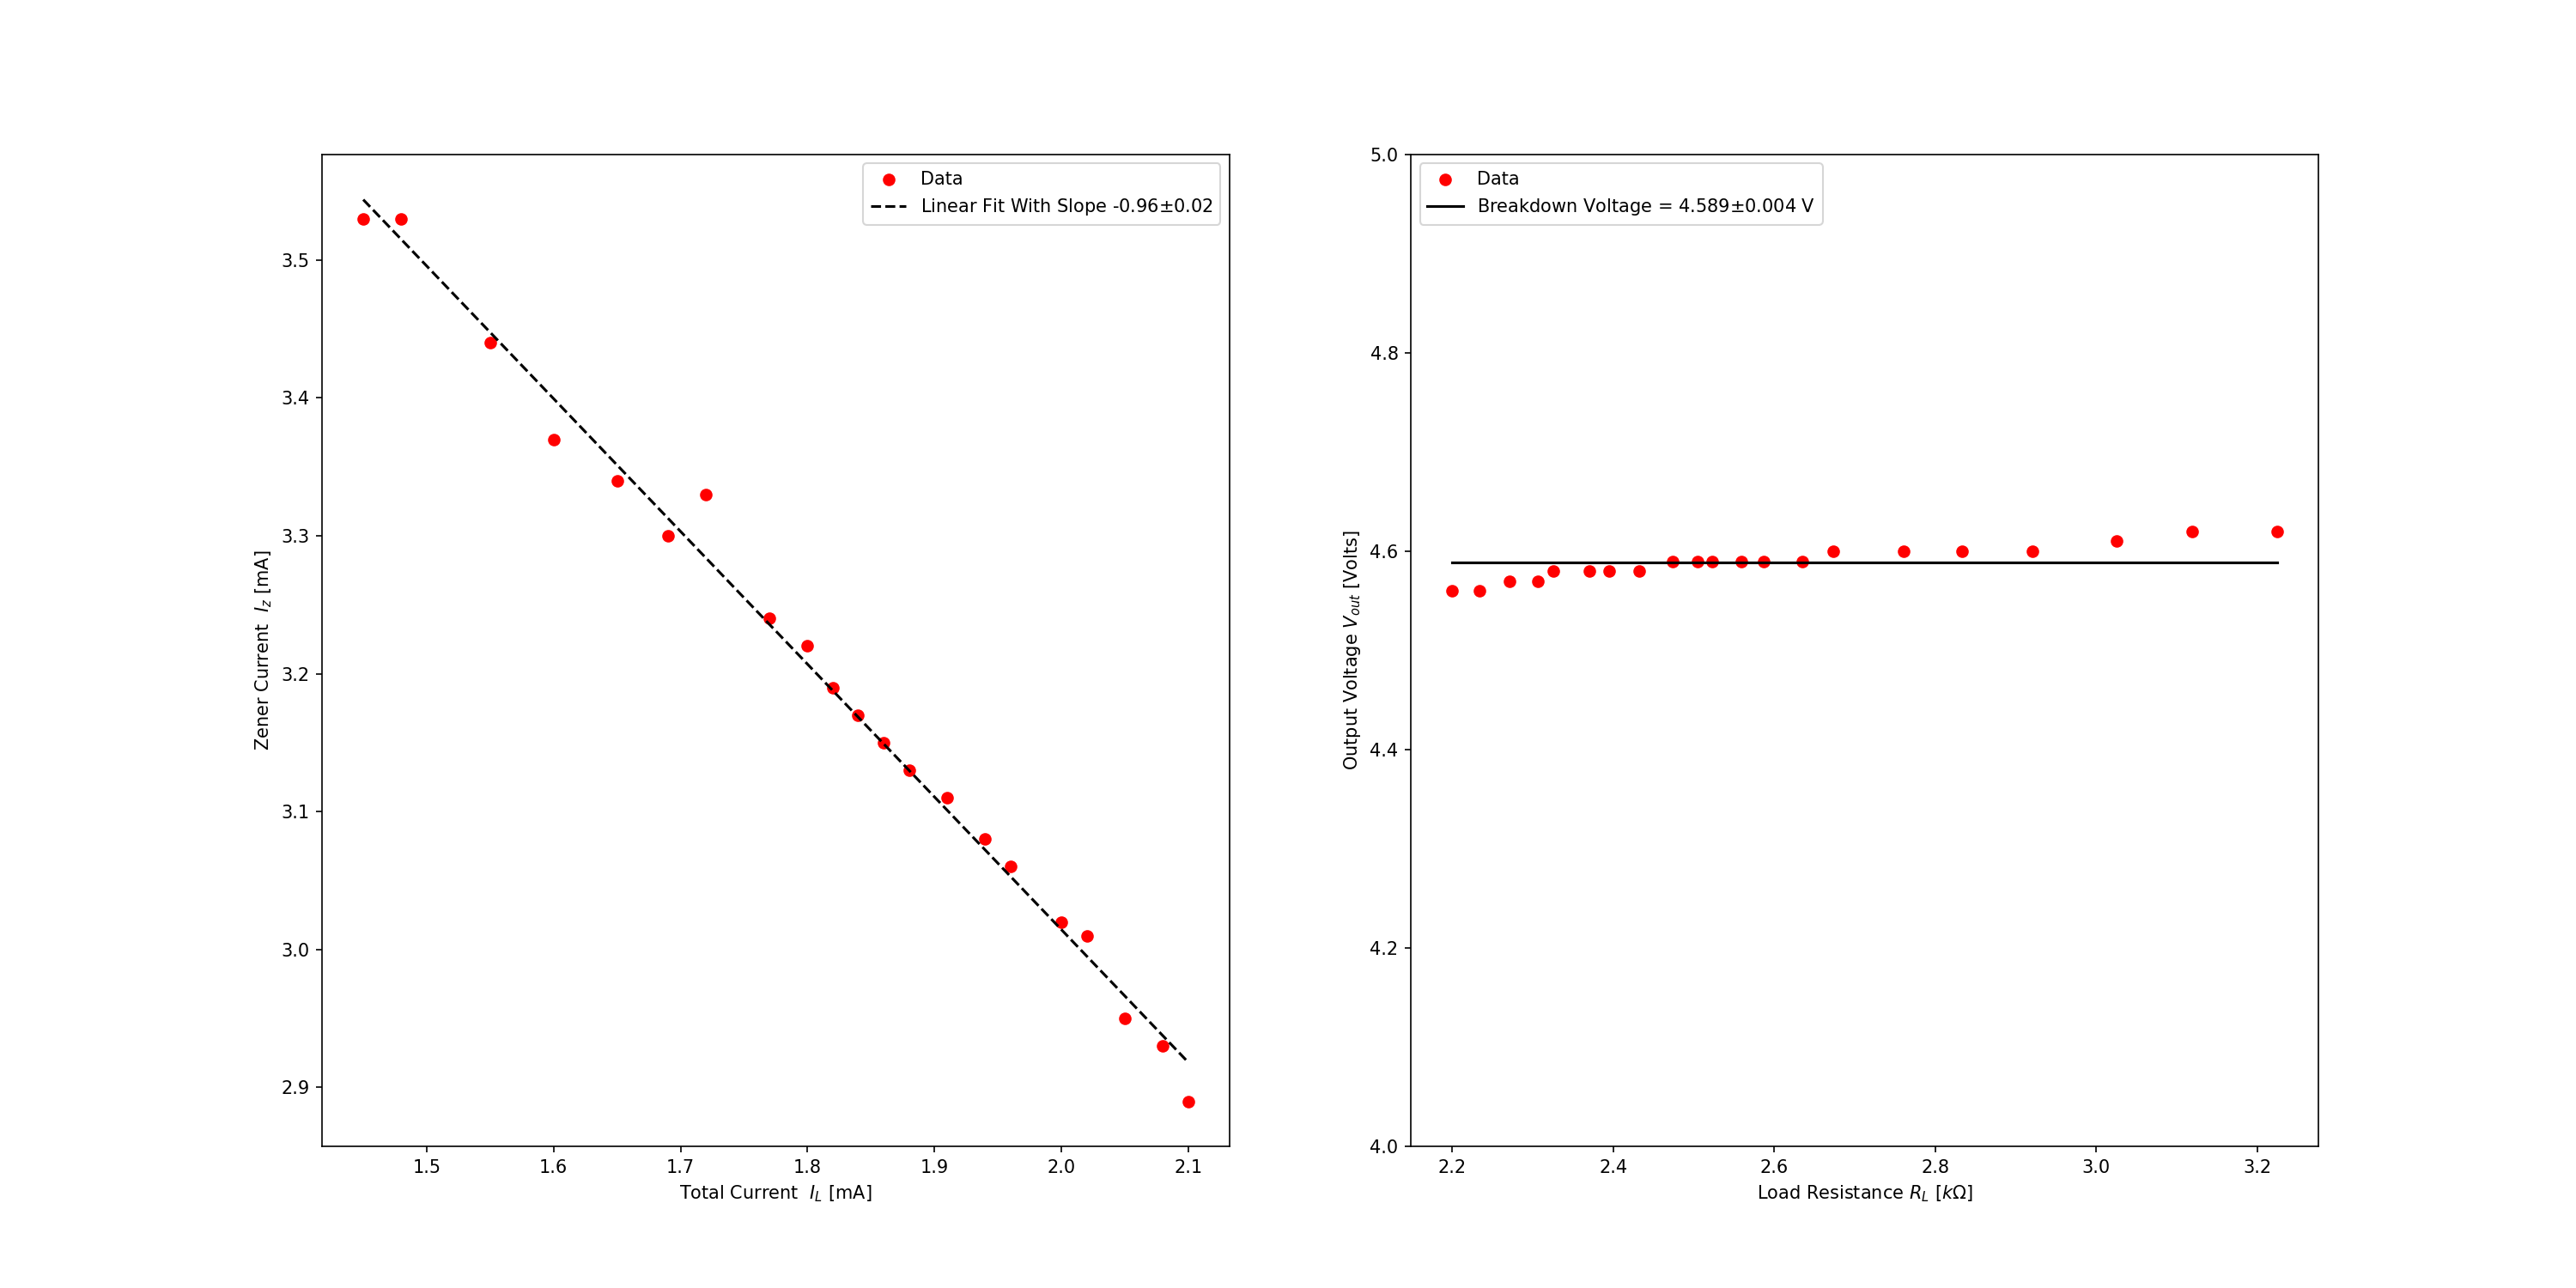
\includegraphics[width=\linewidth]{withrc.png}
    \caption{Plots of the Zener Diode load regulation data with $R_c = 2.2 k\Omega$}
\end{figure}
\begin{align*}
    &\frac{\delta{I_z}}{\delta{I_s}} = -0.96 \pm 0.02 \\ 
    \Rightarrow &\boxed{\delta{I_z} = (-0.96 \pm 0.02)\delta{I_s}}
\end{align*}
From the $V_{in}$ vs $V_{out}$ plot we can see that \textbf{Zener Breakdown} is occurring at $\boxed{V_{out} = 4.589 \pm 0.004 V}$
\clearpage
\section{LM7805 Regulator IC}
In this part of the experiment we studied the properties of the LM7805 Regulator IC.
\subsection{Line Regulation}
Again, as seen before here we varied $V_{in}$ while keeping the load resistance constant at $R_c = 2.2 k\Omega$.
\subsubsection{Data}
\begin{table}[!h]
    \centering
    \caption{Line Regulation data for IC 7805}
    \begin{tabular}{|c|c|c|c|}
    \hline
        \textbf{$R_c$ ($k\Omega$)} & \textbf{$V_{in}$ (V)} & \textbf{$I_L$ (mA)} & \textbf{$V_{out}$ (V)} \\ \hline
        2.2 & 0.1 & 0 & 0 \\ \hline
        2.2 & 0.52 & 0 & 0 \\ \hline
        2.2 & 1 & 0 & 0.0001 \\ \hline
        2.2 & 1.5 & 0.02 & 0.05 \\ \hline
        2.2 & 2.06 & 0.63 & 1.299 \\ \hline
        2.2 & 2.49 & 0.81 & 1.697 \\ \hline
        2.2 & 3.02 & 1.04 & 2.19 \\ \hline
        2.2 & 3.45 & 1.23 & 2.61 \\ \hline
        2.2 & 4.03 & 1.47 & 3.1 \\ \hline
        2.2 & 4.5 & 1.67 & 3.53 \\ \hline
        2.2 & 5.04 & 1.9 & 4.03 \\ \hline
        2.2 & 5.54 & 2.12 & 4.49 \\ \hline
        2.2 & 6.03 & 2.33 & 4.94 \\ \hline
        2.2 & 6.48 & 2.42 & 5.12 \\ \hline
        2.2 & 6.95 & 2.42 & 5.11 \\ \hline
        2.2 & 7.47 & 2.42 & 5.11 \\ \hline
        2.2 & 8 & 2.41 & 5.11 \\ \hline
        2.2 & 8.52 & 2.43 & 5.11 \\ \hline
        2.2 & 9.01 & 2.43 & 5.11 \\ \hline
    \end{tabular}
\end{table}
\subsubsection{Analysis}
Below are the plots generated from the above data.

\begin{figure}[!h]
    \centering
    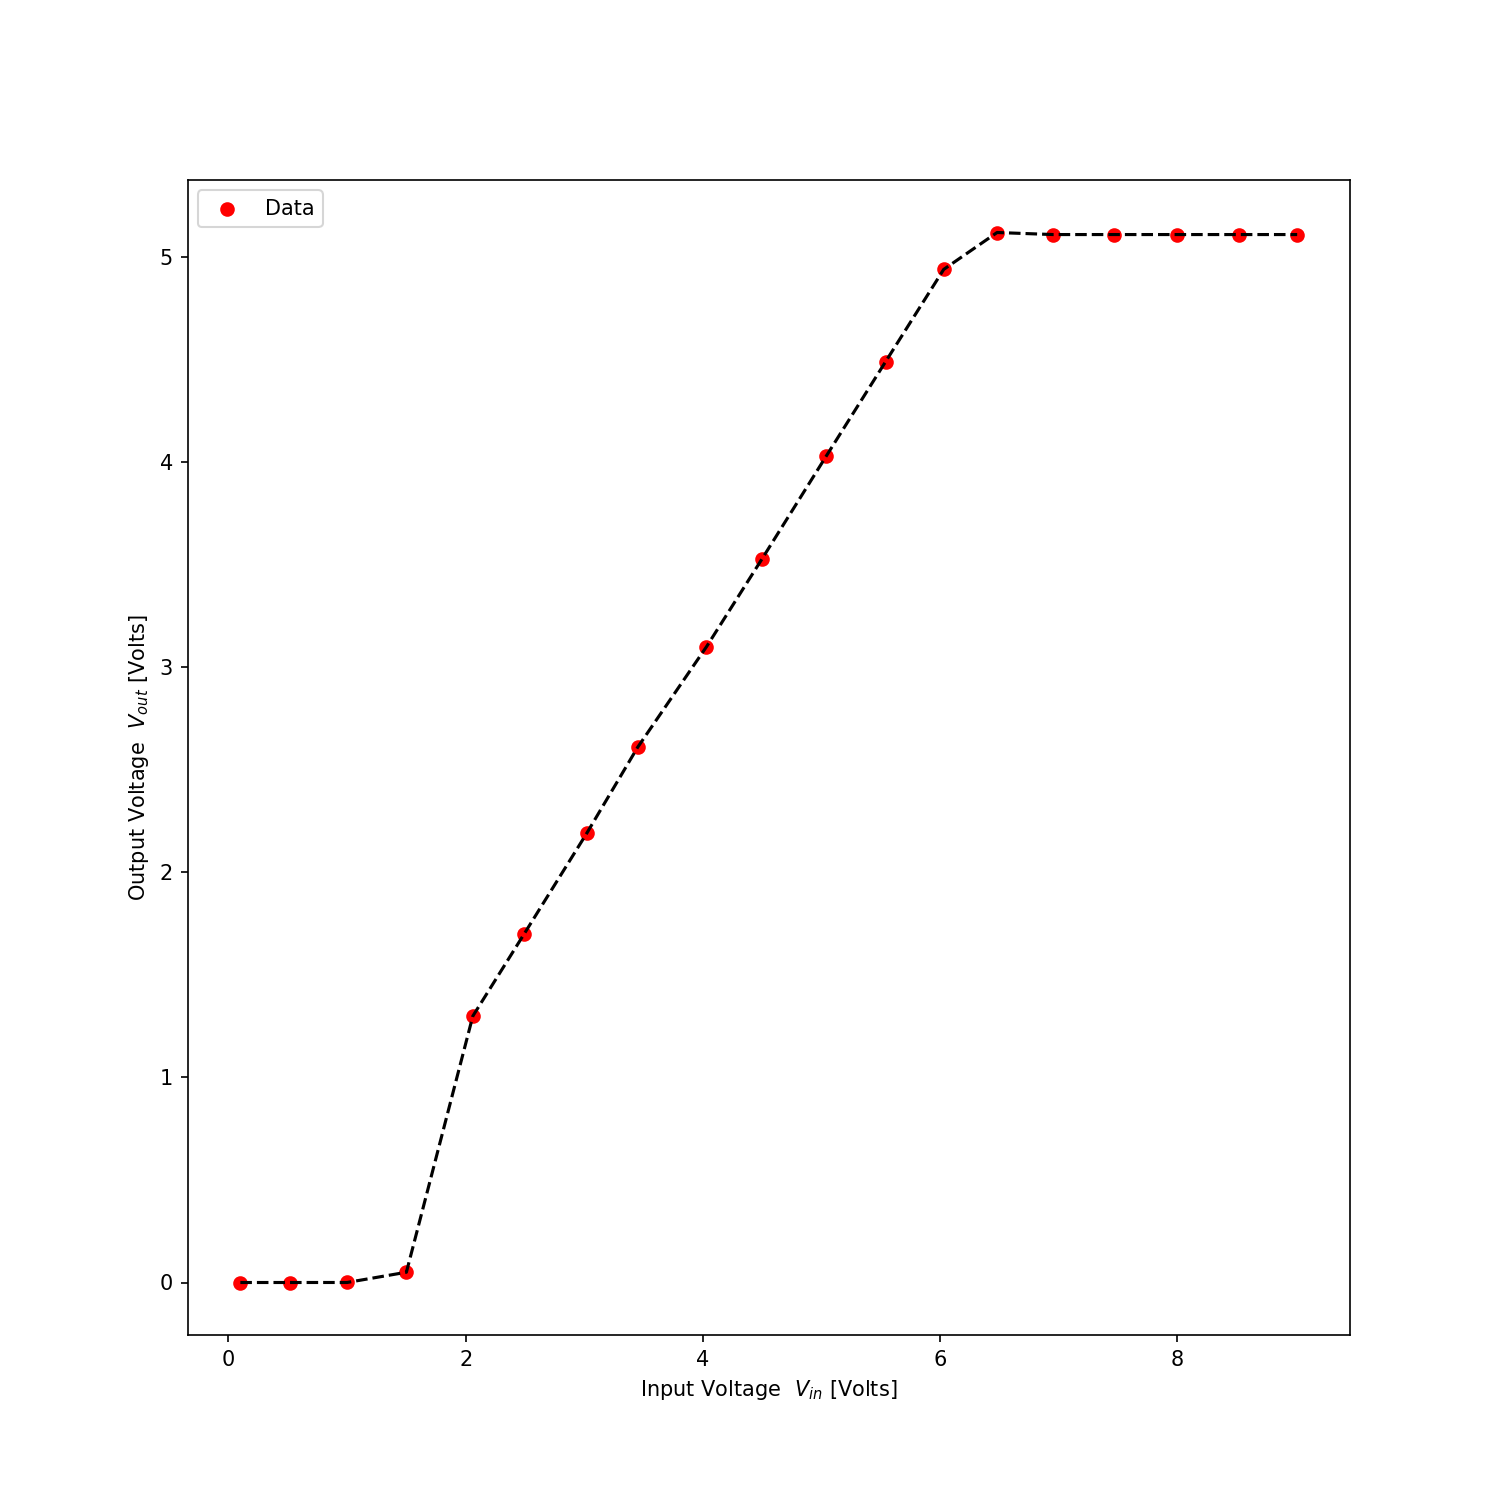
\includegraphics[width=0.45\linewidth]{linereg-ic.png}
    \caption{Plots of the Zener Diode data}
\end{figure}
As we can see from both the data and the plot, the minimum voltage after which
$V_{out}$ was constant was found to be $\boxed{V_{min} = 6.95 V}$
\subsection{Load Regulation}
Again, as seen before here we varied $R_L$ while keeping $V_{in}$ constant at 15 Volts.
The total load resistance is $R_c + R_L = R_L + 2.2 k\Omega$
\subsubsection{Data}
\begin{table}[!h]
    \centering
    \caption{Load Regulation data for IC 7805}
    \begin{tabular}{|c|c|c|c|}
    \hline
        \textbf{$R_L$ ($k\Omega$)} & \textbf{$V_{in}$ (V)} & \textbf{$I_L$ (mA)} & \textbf{$V_{out}$ (V)} \\ \hline
        0 ele& 15 & 2.35 & 5 \\ \hline
        0.072 & 15 & 2.3 & 5.02 \\ \hline
        0.161 & 15 & 2.21 & 5.04 \\ \hline
        0.227 & 15 & 2.15 & 5.03 \\ \hline
        0.312 & 15 & 2.08 & 5.02 \\ \hline
        0.397 & 15 & 2 & 5.01 \\ \hline
        0.508 & 15 & 1.93 & 5.04 \\ \hline
        0.58 & 15 & 1.87 & 5.03 \\ \hline
        0.686 & 15 & 1.78 & 5.03 \\ \hline
        0.809 & 15 & 1.71 & 5.02 \\ \hline
        1.019 & 15 & 1.61 & 5.01 \\ \hline
    \end{tabular}
\end{table}
\subsubsection{Analysis}
Below are the plots generated from the above data.

\begin{figure}[!h]
    \centering
    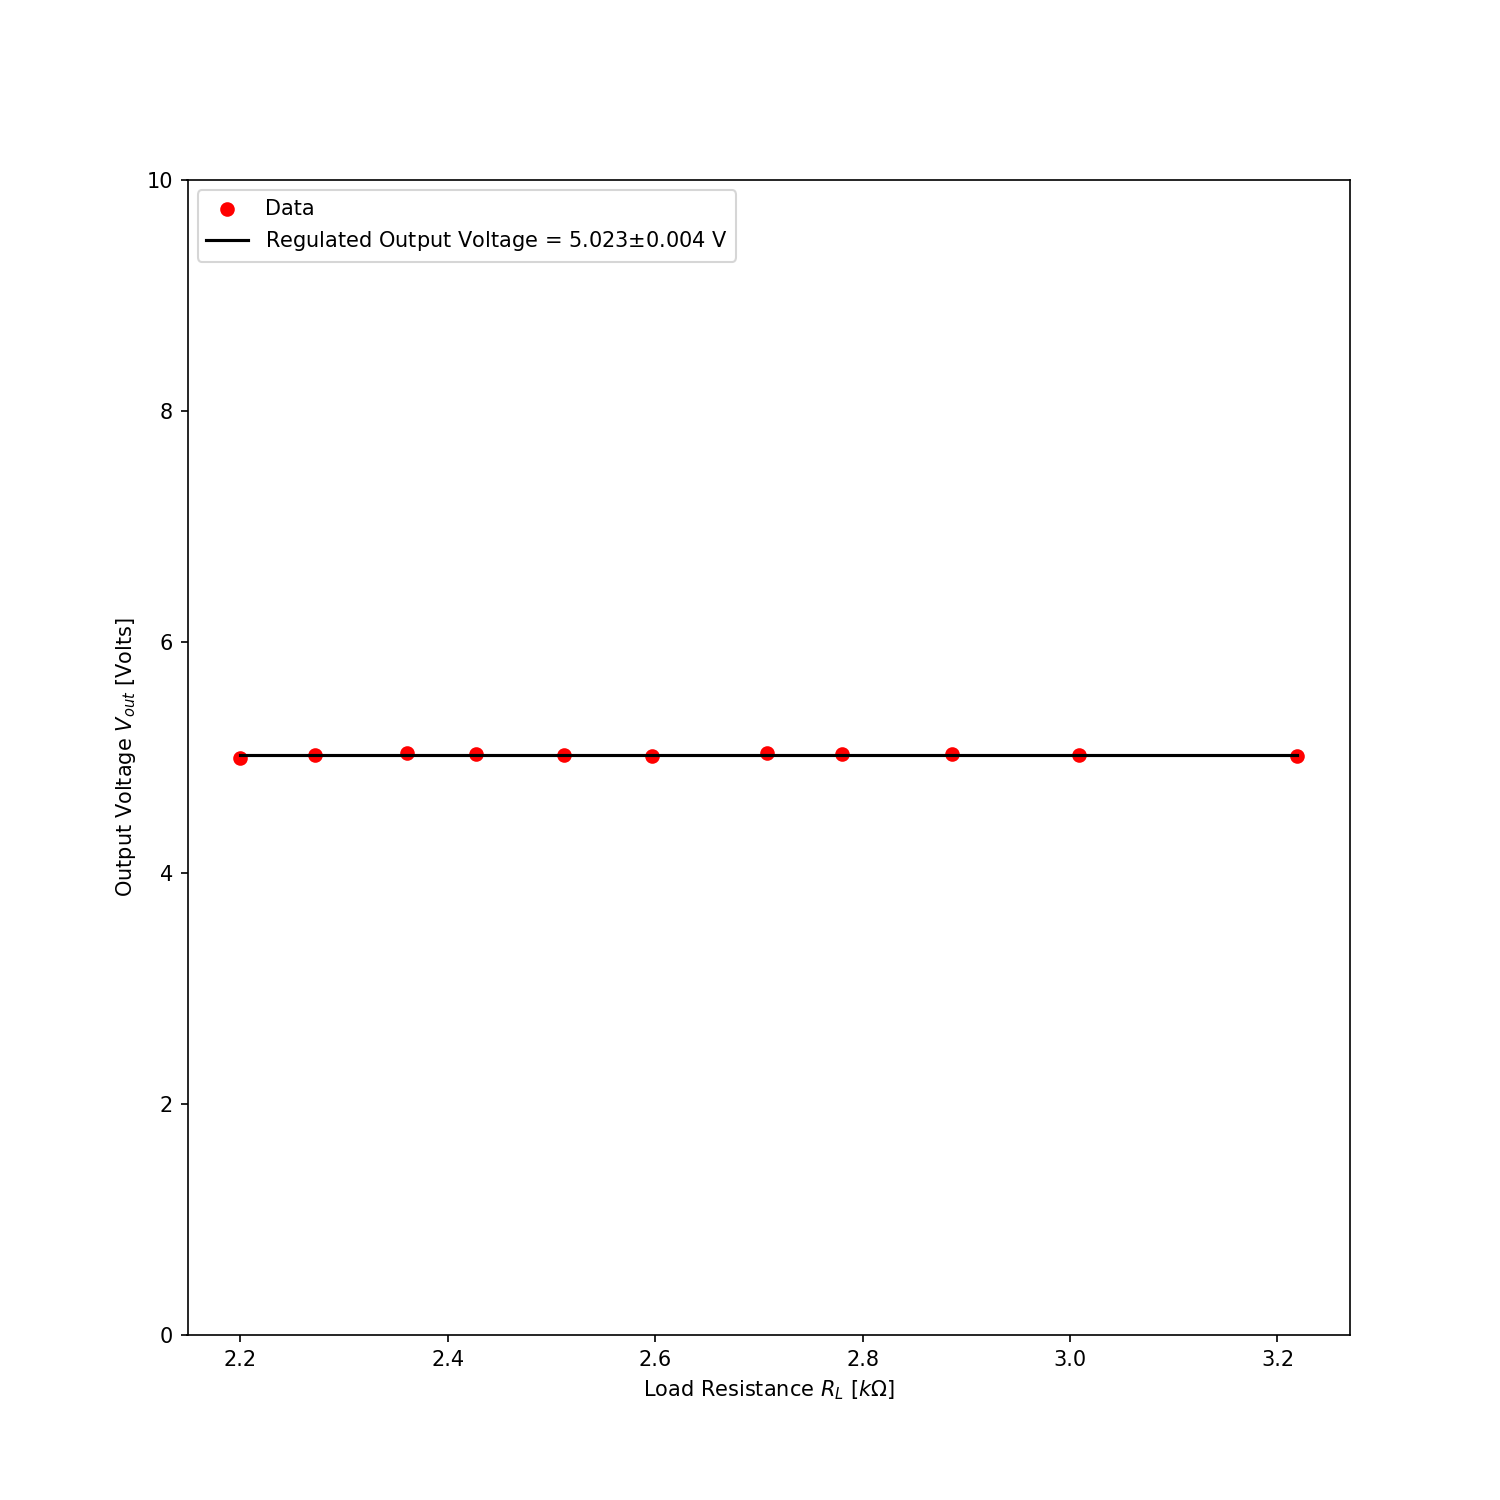
\includegraphics[width=0.5\linewidth]{loadreg-ic.png}
    \caption{Plots of the Zener Diode data}
\end{figure}
From the $V_{in}$ vs $V_{out}$ plot we can see that the output voltage is being 
regulated at $\boxed{V_{out} = 5.023 \pm 0.004 V}$
\clearpage
\section{Conclusion}
In conclusion, in this experiment we looked at how a Zener Diode can be used as a Voltage Regulator, by varying both
the input and the load. We also used the LM7805 Regulator IC, and saw how it is remarkably effective at regulating the output
voltage.
\section{Sources Of Error}
\begin{enumerate}
    \item Loose Contacts between the Breadboard and the components, could lead to fluctuations in measurements.
    \item The multimeters are not ideal ammeters or voltmeters, hence the reading given by them isnt exact. Inaccucies due to
        the finite internal resistance of these devices also leads to some errors in the measurements.
    
\end{enumerate}
\end{document}
